\documentclass{etutez}
\usepackage{graphicx}
\usepackage[toc,page,titletoc]{appendix}
\usepackage[T1]{fontenc}
\usepackage[utf8]{inputenc}
\usepackage[turkish]{babel}
\usepackage{titlesec}
\usepackage{longtable}
\usepackage{mathtools}



\pagenumbering{roman}

\thesistype{M.Sc.} %Yuksek lisans icin M.Sc. doktora icin Ph.D.
\teztipi{Yüksek Lisans}  %Tez tipini yazin

\keywords{FPGA, accelerator, co-processor, OpenCL}
\anahtarsoz{FPGA, hızlandırıcı, yardımcı işlemci, OpenCL}

\title{TITLE OF THE THESIS}
\baslik{FPGA TABANLI SAYISAL S\.{I}NYAL \.{I}\c{S}LEME ALGOR\.{I}TMALARINA \"{O}ZELLE\c{S}T\.{I}R\.{I}LM\.{I}\c{S} YARDIMCI \.{I}\c{S}LEMC\.{I} TASARIMI}  % buyuk harflerle yazilmali

\yazar{ABDULLAH G\.{I}RAY YA\u{G}LIK\c{C}I}    % buyuk harflerle yazilmali
\yazarkucuk{Abdullah Giray Yağlıkçı}    % Soyadi Buyuk harflerle yazilmali
\enstitu{FEN B\.{I}L\.{I}MLER\.{I} } % buyuk harflerle yazilmali
\enstitukucuk{Fen Bilimleri } % kucuk harflerle yazilmali
\institute{Institute of Natural and Applied Sciences}
\bolum{B\.{I}LG\.{I}SAYAR M\"UHEND\.{I}SL\.{I}\u{G}\.{I} } % buyuk harflerle yazilmali
\bolumkucuk{Bilgisayar Mühendisliği } % kucuk harflerle yazilmali
\dept{Computer Engineering}
\supervisor{Assoc. Prof. Oğuz ERG\.{I}N}
\tezyoneticisi{Doç. Dr. Oğuz ERG\.{I}N}
\juribaskani{....}
\juriuyesi{....}
\anablmdalibsk{Doç. Dr. Erdoğan Doğdu}
\enstitumuduru{Prof. Dr. \"Unver KAYNAK}
%\copyrightyear{2001}
\submitdate{August 2014}  % buyuk harflerle yazilmali
\tarih{A\u{G}USTOS 2014}   % buyuk harflerle yazilmali
\tarihkucuk{Ağustos 2014}   % kucuk harflerle yazilmali


\newtheorem{thm}{Theorem}
\newtheorem{preexam}{Example}
\newenvironment{exam} {\begin{preexam}\rm}{\end{preexam}}
\newtheorem{lem}{Lemma}
\newtheorem{proprty}{Property}
\newtheorem{cor}{Corollary}
\newtheorem{defn}{Definition}
\newcommand{\pe}{\preceq}
\newcommand{\po}{\prec}




\hyphenpenalty=5000
\tolerance=1000

\begin{document}


\titlepageMS   % Yuksek lisans tezi kapak sayfasi
%\titlepagePhD    % Doktora tezi kapak sayfasi
%\setcounter{page}{2}
\signaturepageMS  % Yuksek lisans tezi imza sayfasi
%\signaturepagePhD     % Doktora tezi imza sayfasi
\tezbildirimsayfasi    % tez bildirim sayfasi


\begin{ozet}
	Sayısal sinyal işlemede yaygın olarak kullanılan fonksiyonların büyük bir veri seti üzerinde çalıştırılması durumunda paralelleştirilmesi, yürütme zamanını kritik bir şekilde azaltmaktadır. Farklı veriler üzerinde aynı işlemlerin tekrarlandığı algoritmalarda performans artışı sağlamak adına iş parçalarının paralel yürütülebilmesi için çok çekirdekli işlemciler, GPGPU, ASIC tasarımlar ve FPGA tabanlı sistemler algoritmanın koşturulacağı platformların başında gelir. Her bir platformun kendi avantajları ve dezavantajları olmakla beraber, düşük maliyet ile yüksek paralellik sağladığı için GPGPU ve FPGA'ler son yıllarda en yaygın kullanılan platformlardır. Bu tez, ASELSAN - TOBB ETÜ iş birliğinde yürütülen, çıktısı FPGA tabanlı ve OpenCL destekli, ölçeklenebilir ve özelleştirilebilir tasarıma sahip bir yardımcı işlemci ünitesi olan projenin donanım tasarımı kısmını kapsar. Tez çalışmalarına paralel olarak derleyici tasarımı yapılmış fakat tez içeriğine dahil edilmemiştir.
\end{ozet}



\begin{abstract}
	Typical digital signal processing algorithms executes the same DSP functions on different data sets. Parallelizing this process dramatically decreases execution time of such kind of functions. There are 4 popular platforms for parallelized applications: Many-core processors, GPGPUs, ASIC chips and FPGA based applications. Although each kind of platform has own pros and cons, GPGPU and FPGA based applications are more popular than others because of lower price and higher parallel processing capabilities. This MSc thesis consists of hardware design of a project which is managed by ASELSAN and TOBB ETÜ and the output of project is FPGA based OpenCL ready highly scalable and configurable co-processor. Although compiler works are in progress, this thesis only includes the harware design of co-processor.  
\end{abstract}


\begin{tesekkur}
 Bu çalışmayı tamamlamamda emeği geçen değerli danışman hocam Doç. Dr. Oğuz Ergin'e; kıymetli çalışma arkadaşlarım Hasan Hassan, Hakkı Doğaner Sümerkan, Serdar Zafer Can, Serhat Gesoğlu, Volkan Keleş ve Osman Seçkin Şimşek'e; tez çalışmam sırasında beni destekleyen aileme ve değerli arkadaşlarım Fahrettin Koç, Tuna Çağlar Gümüş ve Emrah İşlek'e; projeye desteğinden ötürü ASELSAN'a ve çalışma ortamımızı sağladığı için TOBB ETÜ Mühendislik Fakültesi ve Fen Bilimleri Enstitüsüne teşekkür ederim.
\end{tesekkur}



\pagestyle{plain}




\makeatother




\tableofcontents  
\listoffigures  % Eger tezde herhangi bir sekil yoksa silinmelidir 
\listoftables  % Tezde herhangi bir tablo yoksa silinmelidir
\newpage
\newpage
%\chapter{G\.{I}R\.{I}\c{S}} \label{chapter:giris}
Sayısal sinyal işleme algoritmalarında sıklıkla aynı işlem, farklı veriler üzerinde uygulanmaktadır. Geleneksel işlemcilerde bu tarz bir uygulama her veri için işlemin peşpeşe tekrarlanması ile gerçeklenir. Oysa ki algoritmaların bu özelliği, farklı veriler için uygulanacak aynı işlemin sırayla değil paralel çalıştırılması ile kayda değer performans artışlarını beraberinde getirir. Örneğin N elemanlı iki vektörün skalar çarpımı, N adet çarpma işleminden ve ardından N adet verinin toplanmasından oluşur. N adet çarpma işleminden herhangi birinin bir diğerini beklemeye ihtiyacı yoktur. Bu çarpma işlemlerinin peşi sıra yapıldığı ve paralel yapıldığı durumlar karşılaştırıldığında, paralel olan yöntemde N kata yakın performans artışı gözlenir.Paralelleştirmenin azımsanamayacak performans avantajından dolayı paralel çalışmayı destekleyecek donanım tasarımları üzerinde pek çok çalışma yapılmıştır. Literatürde öne çıkan çalışmaları 4 başlık altında toplamak mümkündür.  \par

Geleneksel işlemcilerde birden fazla iş parçacığının eş zamanlı çalıştırılabilmesi için çok çekirdekli mimari tasarımları yaygın olarak kullanılmaktadır. Çok çekirdekli işlemcilerde bir çekirdek üzerinde 1 veya daha fazla thread koşturulması ile sinyal işleme fonksiyonlarında paralellik sağlanmaktadır. Endüstriyel uygulamalarda kullanılan DSP(Digital Signal Processor) yongaları da çok çekirdekli işlemci mimarisine sahip özelleştirilmiş donanımlardır.\cite{dspArchitectures} Bu tarz mimarilerde çekirdeklerin programlanabilir olması uygulamada esneklik sağlar. Genel amaçlı çok çekirdekli işlemciler, sinyal işleme uygulamalarında alternatiflerine göre daha az paralel ve daha yavaş kalırlarken DSP yongaları, ilave bir donanım olarak donanımın ömrünü kısaltmakta ve güncellenebilirliğini azaltmaktadır.\cite{hallmans2013gpgpu} \par

Bilgisayar ekranına basılacak piksellerin renk ve parlaklık değerlerinin hızlı ve paralel bir biçimde hesaplanabilmesi için geliştirilen grafik işlemcileri çok sayıda çekirdeğe sahiptir.\cite{Kilgariff2005} Hemen her bilgisayarda bulunan grafik işlemcilerinin genel amaçlı paralel hesaplama gerektiren işlerde kullanılması ekonomik ve yüksek performasnlı bir çözüm olarak kendini göstermiştir. Grafik işlemcilerinin genel amaçlı kullanımını destekleyen iki kutup olarak NVidia ve Khronos grubu, sırasıyla CUDA ve OpenCL desteği sağlayarak GPGPU (General Purpose Graphical Processor Unit) kullanımını yaygınlaştırmıştır. \cite{kirk2007nvidia} \cite{stone2010opencl} GPGPU programlama ile uygulamaların paralelleştirilmesi ek donanım gerektirmediği için ekonomik, çok sayıda çekirdekten oluşan donanımlar olduğu için yüksek derecede paralelleştirilebilir bir donanım alternatifidir. Ticari donanımlar olan grafik işlemcilerinin dezavantajı ise birinci önceliği piksel değeri hesaplayan çekirdeklerden oluşması ve çok özel amaçlı işlerde performans bakımından yetersiz kalmasıdır. Burada bahsi geçen yetersizlik buyruk kümesi tasarımı ile ilgilidir.\par

GPGPU ve DSP donanımlarının performans açısından yetersiz kaldığı durumlarda, donanım tasarımına müdahale edilebilen ASIC (Application Specific Integrated Circuit) tasarımlar ve FPGA(Field Programmable Gate Array) tabanlı sistemler ön plana çıkar. ASIC tasarımlar yarı iletken seviyesinde tasarlanan devrelerden oluşurken FPGA tabanlı sistemler, adından da anlaşılacağı üzere, FPGA yongalarında hazır bulunan LUT (Lookup Table), kapılar, bellekler vb. yapılar kullanılarak gerçeklenir. Her iki yaklaşımın diğerlerinden farkı yazılım seviyesinden donanım seviyesine inilmesi ile donanımın uygulamaya özelleştirilerek performans artışının sağlanmasıdır. ASIC - FPGA karşılaştırmasında ASIC uygulamalar daha alt seviyede, FPGA uygulamalar ise daha üst seviyede yapılır. Dolayısıyla ASIC tasarımdan alınan performans artışına FPGA seviyesinde erişilmesi mümkün değildir. Öte yandan ASIC uygulamaların, üretim gerektirdiği için maliyeti fazla, güncellenebilirliği azdır. \cite{kuon2007measuring} \par

Bu tez, sayısal sinyal işleme algoritmalarında yaygın olarak kullanılan fonksiyonların paralel çalıştırılması için tasarlanan FPGA tabanlı bir sistemin donanım tasarımını içerir. Söz konusu sistem ASELSAN ve TOBB ETÜ'nün ortak projesi olup, ASELSAN tarafından sayısal sinyal işleme uygulamalarında kullanılması planlanmaktadır. Dolayısıyla tasarımın temelini oluşturan kriterler ve fonksiyon listesi ASELSAN tarafından belirlenmiştir. \par

Tezin 2. bölümünde ASELSAN tarafından belirlenen tasarım kriterleri ve fonksiyon listesi özetlenmiş ve tasarım öncesi sistem özellikleri belirlenmiştir. 3. bölümde benzer özellikteki mimariler sunulmuş, avantajları ve dezavantajları tartışılmıştır. 4. bölümde buyruk kümesi ve boru hattı tasarımı anlatılmış, 5. bölümde ise mimari tasarımı alt modüllere ayrılarak her bir modülün tasarımı açıklanmıştır. 6. bölümde sonuçların sunumu ile tez sonlandırılmıştır.  
  % Tezin basina kisaltmalar ya da semboller sayfasi konacaks basindaki '%' kaldirilmeli ve semboller.tex dosyasi olusturulmalidir 
\newpage

\setcounter{secnumdepth}{5}
\setcounter{tocdepth}{4}


\pagenumbering{arabic}
\setcounter{page}{1}
\setcounter{section}{1}


\chapter{G\.{I}R\.{I}\c{S}}
Sayısal sinyal işleme algoritmalarında sıklıkla aynı işlem, farklı veriler üzerinde uygulanmaktadır. Geleneksel işlemcilerde bu tarz bir uygulama her veri için işlemin peşpeşe tekrarlanması ile gerçeklenir. Oysa ki algoritmaların bu özelliği, farklı veriler için uygulanacak aynı işlemin sırayla değil paralel çalıştırılması ile kayda değer performans artışlarını beraberinde getirir. Örneğin N elemanlı iki vektörün skalar çarpımı, N adet çarpma işleminden ve ardından N adet verinin toplanmasından oluşur. N adet çarpma işleminden herhangi birinin bir diğerini beklemeye ihtiyacı yoktur. Bu çarpma işlemlerinin peşi sıra yapıldığı ve paralel yapıldığı durumlar karşılaştırıldığında, paralel olan yöntemde N kata yakın performans artışı gözlenir.Paralelleştirmenin azımsanamayacak performans avantajından dolayı paralel çalışmayı destekleyecek donanım tasarımları üzerinde pek çok çalışma yapılmıştır. Literatürde öne çıkan çalışmaları 4 başlık altında toplamak mümkündür.  \par

Geleneksel işlemcilerde birden fazla iş parçacığının eş zamanlı çalıştırılabilmesi için çok çekirdekli mimari tasarımları yaygın olarak kullanılmaktadır. Çok çekirdekli işlemcilerde bir çekirdek üzerinde 1 veya daha fazla thread koşturulması ile sinyal işleme fonksiyonlarında paralellik sağlanmaktadır. Endüstriyel uygulamalarda kullanılan DSP(Digital Signal Processor) yongaları da çok çekirdekli işlemci mimarisine sahip özelleştirilmiş donanımlardır.\cite{dspArchitectures} Bu tarz mimarilerde çekirdeklerin programlanabilir olması uygulamada esneklik sağlar. Genel amaçlı çok çekirdekli işlemciler, sinyal işleme uygulamalarında alternatiflerine göre daha az paralel ve daha yavaş kalırlarken DSP yongaları, ilave bir donanım olarak donanımın ömrünü kısaltmakta ve güncellenebilirliğini azaltmaktadır.\cite{hallmans2013gpgpu} \par

Bilgisayar ekranına basılacak piksellerin renk ve parlaklık değerlerinin hızlı ve paralel bir biçimde hesaplanabilmesi için geliştirilen grafik işlemcileri çok sayıda çekirdeğe sahiptir.\cite{Kilgariff2005} Hemen her bilgisayarda bulunan grafik işlemcilerinin genel amaçlı paralel hesaplama gerektiren işlerde kullanılması ekonomik ve yüksek performasnlı bir çözüm olarak kendini göstermiştir. Grafik işlemcilerinin genel amaçlı kullanımını destekleyen iki kutup olarak NVidia ve Khronos grubu, sırasıyla CUDA ve OpenCL desteği sağlayarak GPGPU (General Purpose Graphical Processor Unit) kullanımını yaygınlaştırmıştır. \cite{kirk2007nvidia} \cite{stone2010opencl} GPGPU programlama ile uygulamaların paralelleştirilmesi ek donanım gerektirmediği için ekonomik, çok sayıda çekirdekten oluşan donanımlar olduğu için yüksek derecede paralelleştirilebilir bir donanım alternatifidir. Ticari donanımlar olan grafik işlemcilerinin dezavantajı ise birinci önceliği piksel değeri hesaplayan çekirdeklerden oluşması ve çok özel amaçlı işlerde performans bakımından yetersiz kalmasıdır. Burada bahsi geçen yetersizlik buyruk kümesi tasarımı ile ilgilidir.\par

GPGPU ve DSP donanımlarının performans açısından yetersiz kaldığı durumlarda, donanım tasarımına müdahale edilebilen ASIC (Application Specific Integrated Circuit) tasarımlar ve FPGA(Field Programmable Gate Array) tabanlı sistemler ön plana çıkar. ASIC tasarımlar yarı iletken seviyesinde tasarlanan devrelerden oluşurken FPGA tabanlı sistemler, adından da anlaşılacağı üzere, FPGA yongalarında hazır bulunan LUT (Lookup Table), kapılar, bellekler vb. yapılar kullanılarak gerçeklenir. Her iki yaklaşımın diğerlerinden farkı yazılım seviyesinden donanım seviyesine inilmesi ile donanımın uygulamaya özelleştirilerek performans artışının sağlanmasıdır. ASIC - FPGA karşılaştırmasında ASIC uygulamalar daha alt seviyede, FPGA uygulamalar ise daha üst seviyede yapılır. Dolayısıyla ASIC tasarımdan alınan performans artışına FPGA seviyesinde erişilmesi mümkün değildir. Öte yandan ASIC uygulamaların, üretim gerektirdiği için maliyeti fazla, güncellenebilirliği azdır. \cite{kuon2007measuring} \par

Bu tez, sayısal sinyal işleme algoritmalarında yaygın olarak kullanılan fonksiyonların paralel çalıştırılması için tasarlanan FPGA tabanlı bir sistemin donanım tasarımını içerir. Söz konusu sistem ASELSAN ve TOBB ETÜ'nün ortak projesi olup, ASELSAN tarafından sayısal sinyal işleme uygulamalarında kullanılması planlanmaktadır. Dolayısıyla tasarımın temelini oluşturan kriterler ve fonksiyon listesi ASELSAN tarafından belirlenmiştir. \par

Tezin 2. bölümünde ASELSAN tarafından belirlenen tasarım kriterleri ve fonksiyon listesi özetlenmiş ve tasarım öncesi sistem özellikleri belirlenmiştir. 3. bölümde benzer özellikteki mimariler sunulmuş, avantajları ve dezavantajları tartışılmıştır. 4. bölümde buyruk kümesi ve boru hattı tasarımı anlatılmış, 5. bölümde ise mimari tasarımı alt modüllere ayrılarak her bir modülün tasarımı açıklanmıştır. 6. bölümde sonuçların sunumu ile tez sonlandırılmıştır.  

\chapter{TEMEL BİLGİLER} \label{chapter:temelBilgiler}
Tez çalışması boyunca kullanılan teknolojiler hakkında temel bilgiler bu bölümde sunulmuştur.
\section{FPGA Platformu}
FPGA'ler birbirlerine programlanabilir bağlantı birimleriyle bağlı matris yapıda özelleştirilebilir mantık bloklarından (Configurable Logic Block/CLB) oluşan programlanabilir yarı iletken devrelerdir. FPGA’ler herhangi bir uygulama için kolayca programlanabilir, aynı FPGA içeriği değiştirilip tekrar programlanarak bir başka uygulama için de kullanılabilir. Bir FPGA’in lojik hücrelerinden oluşan iç mimarisi teorik olarak Şekil \ref{image:fpgaCLB}’de verilmiştir.\par
\begin{figure}[ht]
\centering
\shorthandoff{=}
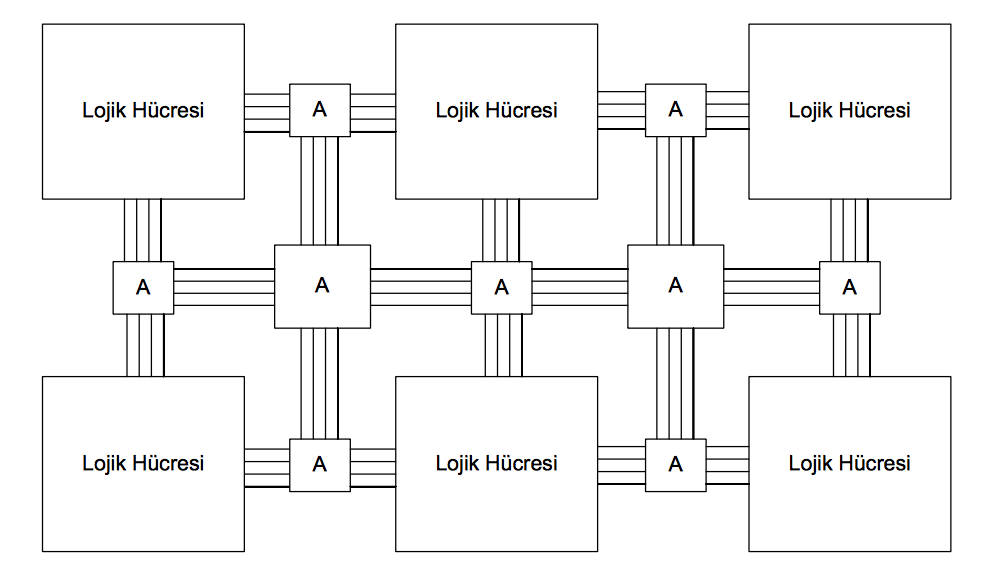
\includegraphics[width=0.8\textwidth]{gorsel/fpgaCLB.png}
\shorthandoff{=}
\caption{FPGA Mantık Hücreleri ve Bağlantı Yapısı}
\label{fpgaCLB}
\end{figure}

FPGA'ler esnek mimari yapıları ve programlanma özellikleri sayesinde kendilerine endüstride hızla yer bulmuştur ve günümüzde de otomotivden, telekomünikasyona, uzay uygulamalarından savunma sanayine ve özellikle yüksek performansla birlikte esneklik isteyen birçok uygulama alanında tercih edilmektedirler. \cite{aykenarThesis} \par

Xilinx ve Altera firmaları dünya üzerinde en çok müşteriye sahip iki firmadırlar. Bu firmalar birçok uygulamaya özel ve farklı ihtiyaçlara hitap eden değişik FPGA aileleri üretmektedirler. Xilinx firmasının piyasada sıklıkla kullanılan farklı FPGA ailelerinden FPGA örnekleri ve özellikleri tablo \ref{table:fpgaModels}’de verilmiştir.\par

\begin{longtable}{p{90pt} p{30pt} p{30pt} p{30pt} p{30pt}}
\caption{Xilinx FPGA Kaynakları} \label{table:fpgaModels} \\
\multicolumn{1}{c}{} & 
\multicolumn{1}{c}{\textbf{Logic Slice}} & 
\multicolumn{1}{c}{\textbf{Block RAM \newline (kb)}} &
\multicolumn{1}{c}{\textbf{DSP Slice}} & 
\multicolumn{1}{c}{\textbf{User I/O}} \\ 
\hline 
\endfirsthead

\multicolumn{2}{c}%
{{\bfseries \tablename \thetable{} -- devam}} \\
\multicolumn{1}{c}{} & 
\multicolumn{1}{c}{\textbf{Logic Slice}} & 
\multicolumn{1}{c}{\textbf{Block RAM (kb)}} &
\multicolumn{1}{c}{\textbf{DSP Slice}} & 
\multicolumn{1}{c}{\textbf{User I/O}} \\  
\hline 
\endhead

\hline \multicolumn{2}{r}{{Sonraki sayfada devam etmektedir.}} \\ 
\endfoot

\hline \hline
\endlastfoot
  Spartan-3A CX3S200A  &   4032 &   288 &  16  &  248 \\
  Spartan-3A CX3S1400A &  25344 &   576 &  32  &  502 \\
  Virtex-5 XC5VLX50    &   9600 &  1152 &  32  &  400 \\
  Virtex-5 XC5VLX330   & 103680 & 10368 &  192 & 1200 \\
  Virtex-7 XC7V585T    & 182100 & 28620 & 1260 &  850 \\
  Virtex-7 XC7V690T    & 108300 & 10888 & 3600 & 1032 \\
  Virtex-7 XC7V2000T   & 305400 & 46512 & 2160 & 1200 \\

\end{longtable}

\newpage
Mantık hücresi (logic slice) olarak isimlendirilen birimler FPGA'lerin işlem ve depolama birimlerini içerir. Bir mantık hücresinin içinde temel olarak 4 veya daha fazla girişli look up table (LUT), 1 adet flip flop ve çeşitli çoklayıcılar bulunur. \par

Basitçe doğruluk tablosunu oluşturabilen sade devreler 1 adet mantık hücresi kullanılarak gerçeklenebilir. Fakat karmaşık mantık yapısına ve çokça yazmaca ihtiyaç duyan devreler ancak birden çok mentık hücresi ile gerçeklenebilirler. \par


Sürekli gelişmekte olan FPGA teknolojisinde artık FPGA yongalarının içerisine özel fonksiyona sahip makro birimler yerleştirilmektedir. Bu makro birimler hard olarak yongaya gömülü durumda olup sadece izin verilen ölçüde parametreleri programlanabilmektedirler. Bu makro bloklara örnek olarak DCM, RAM, DSP slice, çarpıcı birimleri gösterilebilir. Genel olarak bir FPGA’in mimari yapısı şekil \ref{image:fpgaGenelMimari}’de görülebilir.
\begin{figure}[h]
\centering
\shorthandoff{=}
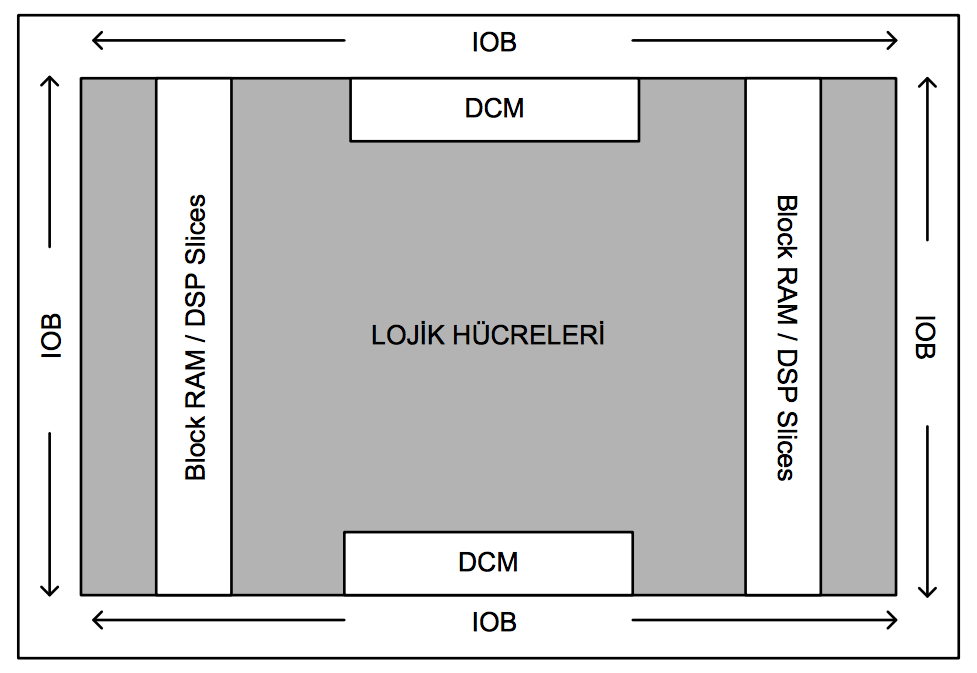
\includegraphics[width=0.8\textwidth]{gorsel/fpgaGenelMimari.png}
\shorthandoff{=}
\caption{FPGA Genel Mimari Yapısı}
\label{fpgaGenelMimari}
\end{figure}
Bu tez çalışması için Xilinx Virtex 7 ailesinden XC7VX690T FPGA’i seçilmiştir. Bu FPGA içinde 108300 slice, 693120 mantık hücresi 866400 CLB flip flop, 10888 KB dağınık ram, 1470 adet 36kbit block ram primitive vardır. \par

\section{GPGPU}

GPU teknolojisindeki ilerlemelerle birlikte, günümüzde kullanılan modern GPU’lar programlanabilir arayüzler sunar hale gelmişlerdir. Bu programlanabilir arayüzler sayesinde GPU’nun işlem gücü ve paralel işleyebilme yeteneği sadece grafik işlemlerinde değil aynı zamanda genel amaçlı hesaplamalarda da kullanılabilir hale gelmiştir. Bu durum ortaya grafik işlem birimi üzerinde genel amaçlı hesaplama (GPGPU - General Purpose programming on Graphic Processing Unit) kavramını çıkarmıştır. \par
GPU’lar yukarıdaki kısımlarda açıklanan işlem hattı mimarisi sayesinde, paralel olarak işlenebilecek nitelikte verinin yüksek performanslı bir şekilde paralel olarak işlenmesi konusunda çok elverişlidirler. GPGPU uygulamaları GPU’ların grafik aygıtlarına özel olan köşe kenar dönüşümü, dokulandırma, renklendirme, gölgelendirme vb. özelliklerinden ziyade SIMD şeklinde çalışan işlem hattı mimarisinden yararlanırlar. GPGPU uygulamaları genel olarak; işaret işleme, ses işleme, görüntü işleme, şifreleme, bioinformatik, yapay sinir ağları, paralelleştirilebilen bilimsel hesaplamalar, istatiksel hesaplamalar gibi yüklü miktarda verinin küçük parçaları üzerinde bağımsız ve paralel olarak işlem yapılmasına uygun olan uygulama alanlarında başarılıdırlar. \cite{ertanYildizThesis}\par

GPGPU uygulamaları genel olarak CPU üzerinde çalışan bir host program ve GPU’daki çekirdekler üzerinde hesaplama yapacak olaran çekirdek fonksiyonundan (kernel function) oluşur. Her çekirdekte çalışan çerkirdek fonksiyonu, stream şekilde GPU’ya iletilen verinin kendine düşen daha küçük bir birimi üzerinde işlem yapar. Giriş verisinin GPU’ya iletilmesi, sonuç verisinin toplanması istenilen formata dönüştürülmesi gibi ardışık işlemleri CPU’da çalışan host program yürütür. \par
\begin{figure}[h]
\centering
\shorthandoff{=}
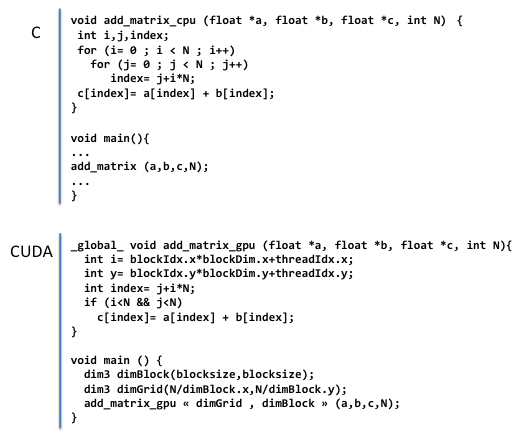
\includegraphics[width=0.9\textwidth]{gorsel/cudaCComparision.png}
\shorthandoff{=}
\caption{CUDA Örnek Kodu}
\label{cudaCComparision}
\end{figure}
Şekil \ref{cudaProgrammingStructure}’da modern GPGPU dillerinden CUDA programlama diline ait programlama modeli yapısı \cite{cudaProgrammingStructure},  Şekil \ref{image:cudaCComparision}’de ise C programlama diliyle yazılmış CPU üzerinde çalışan bir matris toplama fonksiyonu ile yine aynı matris toplama fonksiyonunu GPU üzerinde gerçekleyen, CUDA programlama diliyle yazılmış GPU üzerinde çalışan bir kernel fonksiyonu ve C’de yazılmış bir host program gösterilmiştir. Şekil \ref{cudaProgrammingStructure}’da görüldüğü üzere, CUDA programlama modelinde GPU aygıtı grid olarak görülür ve çok sayıda bloktan oluşur. GPU’da bulunan çok sayıdaki çekirdekten her biri aynı anda bir blok işleyebilir. Bir blok içerisinde paralel olarak çalıştırılabilen çok sayıda thread bulunur. Bu ipliklerinin her biri kendisine düşen veri öbeği üzerinde tanımlanmış olan çekirdek fonksiyonu çalıştırır.

\begin{figure}[h]
\centering
\shorthandoff{=}
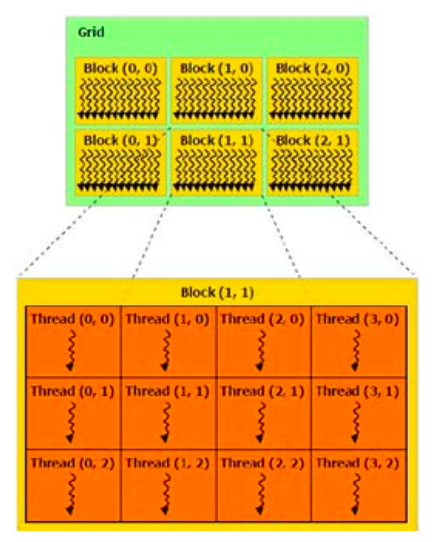
\includegraphics[width=0.7\textwidth]{gorsel/cudaProgrammingStructure.png}
\shorthandoff{=}
\caption{CUDA programlama modeli}
\label{cudaProgrammingStructure}
\end{figure}

% first column





Tablo \ref{table:cudaCComparision}’de görüldüğü gibi C programlama dilinde yazılmış olan matris toplama fonksiyonu matris elemanları üzerinde ardışık döngüler şeklinde işlem yaparak matris toplama işlemini gerçekleştirir. CUDA ile yazılmış matris toplama programına bakıldığında, program CPU üzerinde çalışan host programdaki main fonksiyonundan ve GPU üzerinde çalışan add\_matrix\_gpu çekirdek fonksiyonundan oluşur. Host program bir bloğun boyutunu ve grid içerisindeki blok sayısını belirler. Daha sonra bloklar üzerinde paralel olarak çalışacak olan add\_matrix\_gpu fonksiyonunu çağırır. çağrı sonucu add\_matrix\_gpu çekirdek fonksiyonu bloklar ve bloklardaki threadler üzerinde paralel olarak yürütülür. Her bir thread kendi thread numarası (thread ID), blok numarası (block ID) ve blok boyutunu (blockDim) kullanarak kendine düşen veri parçası için matris toplama işlemini gerçekleştirir. \par



\chapter{DENEYSEL \c{C}ALI\c{S}MA }

\chapter{DE\u{G}ERLEND\.{I}RME }

\chapter{SONU\c{C}}


\newpage
\pagestyle{plain}
\addcontentsline{toc}{chapter}{\numberline{KAYNAKLAR}}


\begin{thebibliography}{99}

\bibitem{cudaProgrammingStructure} Lippert, A. (2009). NVIDIA GPU Architecture for General Purpose Computing, 18.

\bibitem{dspArchitectures} Edwin. J. Tan, Wendi. B. Heinzelman. 2003. DSP Architectures: Past, Present and Futures. ACM Sigarch Computer Architecture News

\bibitem{hallmans2013gpgpu} Hallmans, Daniel, et al. 2013. GPGPU for industrial control systems. IEEE 18th Conference on Emerging Technologies \& Factory Automation ETFA

\bibitem{Kilgariff2005} Emmett Kilgariff and Randima Fernando. 2005. The GeForce 6 series GPU architecture. In ACM SIGGRAPH 2005 Courses SIGGRAPH '05, John Fujii (Ed.). ACM, New York, NY, USA

\bibitem{kirk2007nvidia} Kirk, D. 2007. NVIDIA CUDA software and GPU parallel computing architecture. ISMM Vol. 7, pp. 103-104

\bibitem{stone2010opencl} Stone, J. E., Gohara, D., \& Shi, G. 2010. OpenCL: A parallel programming standard for heterogeneous computing systems. Computing in science \& engineering, 12(3), 66

\bibitem{kuon2007measuring} Kuon, I., \& Rose, J. 2007. Measuring the gap between FPGAs and ASICs. Computer-Aided Design of Integrated Circuits and Systems, IEEE Transactions on, 26(2), 203-215.

\bibitem{smith1997matlab}Smith, R.L., \"The MATLAB project book for linear algebra\", 1997 Prentice Hall

\bibitem{cooleyTukey} Cooley, J. W., \& Tukey, J. W. (1965). An algorithm for the machine calculation of complex Fourier series. Mathematics of computation, 19(90), 297-301.

\bibitem{eigenvalueComputation} Gotze, J.; Paul, S.; Sauer, M., \"An efficient Jacobi-like algorithm for parallel eigenvalue computation,\" Computers, IEEE Transactions on , vol.42, no.9, pp.1058,1065, Sep 1993

\bibitem{flynnTaxonomy}Flynn, M. J. (September 1972). \"Some Computer Organizations and Their Effectiveness\". IEEE Trans. Comput. C–21 (9): 948–960. doi:10.1109/TC.1972.5009071

\bibitem{shivakumar2002modeling} Shivakumar, P., Kistler, M., Keckler, S. W., Burger, D., \& Alvisi, L. (2002). Modeling the effect of technology trends on the soft error rate of combinational logic. In Dependable Systems and Networks, 2002. DSN 2002. Proceedings. International Conference on (pp. 389-398). IEEE.

\bibitem{seiler2008larrabee} Seiler, L., Carmean, D., Sprangle, E., Forsyth, T., Abrash, M., Dubey, P., ... \& Hanrahan, P. (2008). Larrabee: a many-core x86 architecture for visual computing. ACM Transactions on Graphics (TOG), 27(3), 18.

\bibitem{molka2009memory} Molka, D., Hackenberg, D., Schone, R., \& Muller, M. S. (2009, September). Memory performance and cache coherency effects on an Intel Nehalem multiprocessor system. In Parallel Architectures and Compilation Techniques, 2009. PACT'09. 18th International Conference on (pp. 261-270). IEEE

\bibitem{hackenberg2009comparing} Hackenberg, D., Molka, D., \& Nagel, W. E. (2009, December). Comparing cache architectures and coherency protocols on x86-64 multicore SMP systems. InProceedings of the 42Nd Annual IEEE/ACM International Symposium on microarchitecture (pp. 413-422). ACM

\bibitem{MCSE.2012.23} Heinecke, A., Klemm, M., Bungartz H.J., \"From GPGPU to Many-Core: Nvidia Fermi and Intel Many Integrated Core Architecture\" Computing in Science and Engineering, vol. 14, no. 2, pp. 78-83, March-April, 2012 

\bibitem{cpuGpuMemoryTable} http://supercomputingblog.com/cuda/cuda-memory-and-cache-architecture/

\bibitem{tileArchitecture} Wentzlaff, D., Griffin, P., Hoffmann, H., Bao, L., Edwards, B., Ramey, C., Mattina, M., Miao, C.-C., III, J. F. B. \& Agarwal, A. (2007). On-Chip Interconnection Architecture of the Tile Processor.. IEEE Micro, 27, 15-31. 

\bibitem{nvidiaPTXISA} http://docs.nvidia.com/cuda/parallel-thread-execution/\#texture-instructions

\bibitem{x86ISA} http://en.wikipedia.org/wiki/X86\_instruction\_listings

\bibitem{MIPSISA} http://www.mrc.uidaho.edu/mrc/people/jff/digital/MIPSir.html

\bibitem{superscalar600mhz} Gieseke, B. A., Allmon, R. L., Bailey, D. W., Benschneider, B. J., Britton, S. M., Clouser, J. D., ... \& Wilcox, K. E. (1997, February). A 600 MHz superscalar RISC microprocessor with out-of-order execution. In Solid-State Circuits Conference, 1997. Digest of Technical Papers. 43rd ISSCC., 1997 IEEE International (pp. 176-177). IEEE.

\bibitem{superscalarpatent}Garg, S., Hagiwara, Y., Lau, T. L., Lentz, D. J., Miyayama, Y., Trang, Q. H., ... \& Wang, J. (1996). U.S. Patent No. 5,560,032. Washington, DC: U.S. Patent and Trademark Office.

\bibitem{interleavedMultithreading} Laudon, J., Gupta, A., \& Horowitz, M. (1994). Interleaving: A multithreading technique targeting multiprocessors and workstations. ACM SIGPLAN Notices, 29(11), 308-318.

\bibitem{Controldatacorp}Control Data Corp, «CDC Cyber 170 Computer Systems; Models 720, 730, 750, and 760; Model 176 (Level B); CPU Instruction Set; PPU Instruction Set,» pp. 2-44.

\bibitem{TeraMTA}A. e. a. Snavely, \"Multi-processor Performance on the Tera MTA,\" in IEEE Computer Society Proceedings of the 1998 ACM/IEEE conference on Supercomputing, 1998. 


\end{thebibliography} % Kaynakca .bib seklinde degil de kaynakca.tex dosyasi olarak hazirlanirsa bu satir kullanilmali
%\bibliography{kaynakca} % kaynakca.bib dosyasi hazirlanirsa bu satir kullanilmali
%\bibliographystyle{abbrv} % kaynakca.bib ile beraber kullanim icin.
%\renewcommand{\appendixname}{}
\renewcommand{\appendixtocname}{EKLER}
\renewcommand{\appendixpagename}{EKLER}

\begin{appendices}
\appendix
\chapter{Veriler}



\chapter{Algoritma}
\end{appendices}
\newpage
\pagestyle{plain}
\addcontentsline{toc}{chapter}{\numberline{\"OZGE\c{C}M\.{I}\c{S}}}
\begin{center}
{\LARGE \bf \"OZGE\c{C}M\.{I}\c{S}}
\end{center}
\vspace{0.5cm}
{\bf Ki\c{s}isel Bilgiler}


\noindent
\begin{tabular}{@{}lll@{}}
Soyad{\i}, Ad{\i} & : Yağlıkçı, Abdullah Giray &\\
Uyru\u{g}u & : T.C.&\\
Do\u{g}um tarihi ve yeri & : 09.08.1988 Ankara&\\
Medeni hali & : Bekar& \\
Telefon & : &\\
Faks & : &\\
e-mail & : agyaglikci@.etu.edu.tr &\\
\end{tabular}

\vspace{0.5cm}
\noindent
{\bf E\u{g}itim}


\noindent
\begin{tabular}{@{}llc@{}}
{\bf Derece} & {\bf E\u{g}itim Birimi} & {\bf Mezuniyet Tarihi}\\
Y. Lisans & TOBB Ekonomi ve Teknoloji \"Universitesi & 2014\\
Lisans & TOBB Ekonomi ve Teknoloji \"Universitsi& 2011\\
\end{tabular}

\vspace{0.5cm}
\noindent
{\bf \.{I}\c{s} Deneyimi}


\noindent
\begin{tabular}{@{}lll@{}}
{\bf Y{\i}l} & {\bf Yer} & {\bf G\"orev}\\
2012-2014 & TOBB Ekonomi ve Teknoloji \"Universitesi & Burslu Yüksek Lisans Öğrencisi\\
\end{tabular}

\vspace{0.5cm}
\noindent
{\bf Yabanc{\i} Dil}


\noindent
\begin{tabular}{@{}l@{}}
\.{I}ngilizce (İleri Seviye)\\
\end{tabular}


\vspace{0.5cm}
\noindent
{\bf Yay{\i}nlar} \\
\noindent
Mustafa Cavus, Hakki Doganer Sumerkan, Osman Seckin Simsek, Hasan Hassan, Abdullah Giray Yaglikci, Oguz Ergin: GPU based Parallel Image Processing Library for Embedded Systems. VISAPP 2014




\end{document}
